\subsection{Quadrupole Scans}
\label{03_2_QuadScans}
\tb{Taken from Davide's IPAC17 paper MOPAB115}
%Davides IPAC17 2017  MOPAB115

Quadrupolar Scan technique was employed to measure emittance and Twiss parameters with help of 
a profile monitors~\ref{01_MTV}.
It is one of the main methods routinely employed in 
relativistic beams in transfer lines, and it is extensively documented in the literature 
(e.g. in~\cite{Lohl2005}).
Here we recall only the basic principles for the simplest case of a
linear and uncoupled transfer line,
where one can treat the horizontal and vertical phase-spaces
independently using a 2D matrix formalism.
%
%For 4D reconstruction of the transverse phase space one can see, for example, ~\cite{}.
A quadrupole scan consists in reconstructing the transverse phase-space
distribution at some location along a beam line by measuring the beam
profile downstream.
In linear optics the transfer matrix from a \emph{reconstruction} (R)
to a \emph{measurement} (M) location can be written as:
%
\begin{align}
\begin{pmatrix}
x \\
x'
\end{pmatrix}_M
&=
\begin{bmatrix}
A & B \\
C & D
\end{bmatrix}
\begin{pmatrix}
x \\
x'
\end{pmatrix}_R
\label{eq:simpleTranport}
\end{align}
where $A$, $B$, $C$, $D$ are coefficients that depends on the layout of
the beam line and on the strength of its quadrupoles. 
%
The beam variance ($\sigma_M^2$) at the measurement location can be
expressed as a function of the Twiss parameters $\alpha_R$, $\beta_R$
and $\gamma_R$ at the reconstruction location as:
%
\begin{align}
 \sigma_M^2 = \beta_M \epsilon &= 
 \begin{pmatrix}
  A^2 & -2AB & B^2 
  \end{pmatrix} 
\begin{pmatrix}
   \beta_R \\
   \alpha_R \\
   \gamma_R
\end{pmatrix}
\epsilon
\label{eq:varianceForQuadscan}
\end{align}
%
where $\epsilon$ is the beam \emph{geometric} emittance.
Further we will use the \emph{normalised}
emittance definition $\epsilon_N = \epsilon \, \gamma_{\text{rel}}$
where $\gamma_{\text{rel}}$ is the relativistic factor. 
\todo[inline]{\textepsilon for geometric or normalized?}
\tr{Piotr: I think it will be easier to leave \textepsilon~ for normalized and define here $\epsilon_G$ for geometric.
Otherwise in all the plots and tables we need to stick N next to epsilon.}
%
One can measure the beam variance $\sigma_{M,i}^2$ (e.g. with an
intercepting screen as normally done at CTF3)
while varying the strength of the quadrupoles and therefore the
coefficients of the transfer matrix, 
and so solve linear system of equations:
%
\begin{align}
\begin{pmatrix}
\sigma_{M,1}^2 \\
\sigma_{M,2}^2 \\
\vdots \\
\sigma_{M,n}^2
\end{pmatrix}
&=
\begin{pmatrix}
\beta_{M,1} \\
\beta_{M,2} \\
\vdots \\
\beta_{M,n}
\end{pmatrix}
\epsilon 
= 
 \begin{pmatrix}
  A_1^2 & -2A_1B_1 & B_1^2 \\
  A_2^2 & -2A_2B_2 & B_2^2 \\
  \vdots & \vdots & \vdots \\
  A_n^2 & -2A_nB_n & B_n^2 \\
  \end{pmatrix} 
\begin{pmatrix}
  \beta_R \\
  \alpha_R \\
  \gamma_R
\end{pmatrix}
\epsilon.
\label{eq:dataCollectionQuadscan}
\end{align}
%
Finally by knowing that the Twiss parameters must satisfy the relation
$\beta\gamma - \alpha^2 = 1$, one can disentangle and obtain both the
beam emittance and the Twiss parameters at the reconstruction location.

%%%%%%%%%%%%%%%%%%%%%%%%%%%%%%%%%%%%%%%%%%%%%%%%%%%%%%%%%%%%%%%%%%%%%%%%%%%%%%%%%%%%%%%%%%%%%%%%%%%%%
%%%%%%%%%%%%%%%%%%%%%%%%%%%%%%%%%%%%%%%%%%%%%%%%%%%%%%%%%%%%%%%%%%%%%%%%%%%%%%%%%%%%%%%%%%%%%%%%%%%%%
%%%%%%%%%%%%%%%%%%%%%%%%%%%%%%%%%%%%%%%%%%%%%%%%%%%%%%%%%%%%%%%%%%%%%%%%%%%%%%%%%%%%%%%%%%%%%%%%%%%%%

\subsubsection{Constant beam size}

The necessary condition for obtaining a good fit is that the matrix in
Eq.~\ref{eq:dataCollectionQuadscan} is well conditioned. 
A standard way is to vary a single quadrupole strength such that the
beam size at the measurement location goes through a minimum. 
However this is not necessary, and sometimes one might want to keep the
beam size constant or within a certain range due to limitations of the
measurement device (e.g. poor resolution or field of view of the screen
used).
This was already exploited at the former CLIC Test Facility 2 (CTF2) in
\cite{Tenenbaum1997} and used elsewhere, e.g. in \cite{prat2014}.
Here one needs an initial estimate of the Twiss parameters that are
going to be measured, and so build a well conditioned matrix of the
coefficients in Eq.~\ref{eq:dataCollectionQuadscan} according to the
given constraint.

At CTF3 we use the MATLAB \emph{fsolve} solver \cite{mat:solver} for
setting up such a measurement.
Figure~\ref{fig:constantBeam} shows a comparison of two measurement
performed on the Drive Beam at CTF3.
The first one, in blue, has been obtained by varying only one
quadrupole, while three quadrupoles have been used for the measurement
in red.
The second measurement, using the Twiss parameters measured from the
first one, was set up trying to keep the beam size constant at the
screen.
The fitted Twiss parameters are reported in
Table~\ref{tab:constantBeam}.
%
\begin{figure}[htb]
   \centering
   \includegraphics*[width=0.6\columnwidth]{MOPAB115f3.eps}
   \caption{Horizontal beam variance $\sigma_{xx}$ measured at the screen for different settings of quadrupole settings. Dashed are the expected values from the fitted Twiss parameters.}
   \label{fig:constantBeam}
\end{figure}
%
%
\begin{table}[bt]
   \centering
   \begin{tabular}{ l c c c c c}
    \hline                
                & $\beta_x$ [m]      & $\alpha_x$          & $\epsilon_{Nx}$ [$\mu$mm] \\
  %Normal       & $5.02\pm0.19$      & $-3.53\pm0.14$      & $155\pm3$ \\
  %Constant     & $3.98\pm0.17$      & $-2.64\pm0.12$      & $146\pm3$ \\
  Standard      & $5.0\pm0.2$        & $-3.5\pm0.1$        & $155\pm3$ \\
  Constant size & $4.0\pm0.2$        & $-2.6\pm0.1$        & $146\pm3$ \\
    \hline
   \end{tabular}
   \caption{Twiss Parameters Fitted from the Measurements Shown in Fig.~\ref{fig:constantBeam}}
   \label{tab:constantBeam}
\end{table}
%
Note that the fitted Twiss parameters, while being not too far, are not
fully consistent.
This is believed to be due to the Gaussian fit that is applied to the
measured profiles, which sometimes can be far from being Gaussian as
shown later in Fig.~\ref{fig:tomo}~\protect\subref{fig:tomoprofiles}.
%%%% Could be added:
This provide also an idea of the accuracy of such a measurement. 
The experience at CTF3 is that when comparing the Twiss parameters of
two different beam setups it is good practice to use the same scan
settings. This allows to minimise the systematic errors when comparing
the obtained values.
%%%%
Probably due to a systematic error on the measurement which has not
been revealed yet. 
This inconsistency have been observed several times at this location
while using different quadrupole scan ranges.

%%%%%%%%%%%%%%%%%%%%%%%%%%%%%%%%%%%%%%%%%%%%%%%%%%%%%%%%%%%%%%%%%%%%%%%%%%%%%%%%%%%%%%%%%%%%%%%%%%%%%
%%%%%%%%%%%%%%%%%%%%%%%%%%%%%%%%%%%%%%%%%%%%%%%%%%%%%%%%%%%%%%%%%%%%%%%%%%%%%%%%%%%%%%%%%%%%%%%%%%%%%
%%%%%%%%%%%%%%%%%%%%%%%%%%%%%%%%%%%%%%%%%%%%%%%%%%%%%%%%%%%%%%%%%%%%%%%%%%%%%%%%%%%%%%%%%%%%%%%%%%%%%


\subsection{Transverse matching}
%
In an ideal machine the beam is passing through the centre of the quadrupoles, 
therefore the beam centroid should not move while performing a quadrupole scan.
In practice this is not always the case,
but the movement of the beam centroid at the measurement location ($x_{M,i}$) 
can be used to fit the centroid phase-space coordinates ($x_R, x'_R$) 
by inverting the following system of equations: 
\begin{equation}
\begin{pmatrix}
  x_{M,1} \\
  x_{M,2} \\
  \vdots \\
  x_{M,n} 
\end{pmatrix}
= 
 \begin{pmatrix}
  A_1 & B_1 \\
  A_2 & B_2 \\
  \vdots & \vdots \\
  A_n & B_n \\
  \end{pmatrix} 
\begin{pmatrix}
  x_R \\
  x'_R 
\end{pmatrix}.
\label{eq:dataCollectionCentroide}
\end{equation}
%
Moreover, starting from the Twiss parameters and assuming Gaussian beams, 
one can represent the beam phase-space distribution as an ellipse of equation:
%
\begin{align}
\epsilon_x &= \gamma_x \, x^2 + 2 \alpha_x \, x \, x' + \beta_x \, x'^2.
\end{align}
%

At CTF3 the first recombination takes place into the Delay Loop (DL): 
half of the beam is \emph{delayed}, while the other half \emph{bypass} the DL. 
Both are then recombined in the following transfer line. 
Figure~\ref{fig:DLClosure} shows the ellipse representation in phase-space of 
a typical well matched delayed beam, bypass beam and 
relative factor two combined beam measured at CTF3.
The measured Twiss parameters and centroid coordinate are reported in Table~\ref{tab:DLClosure}.
%
\begin{figure}[htb]
   \centering
   \includegraphics*[width=0.6\columnwidth]{MOPAB115f2.eps}
   \caption{Phase-space representation of a bypass (red), delayed (blue) and combined (green) beam 
            for an example measurement at CTS. 
            Dashed are the expected nominal ellipses assuming the measured emittances.}
   \label{fig:DLClosure}
\end{figure}
%
\begin{table*}[bt]
   \centering
   \caption{Beam Centroid and Twiss Parameters Related to Fig.~\ref{fig:DLClosure}}
   \begin{tabular}{ l c c c c c}
    \hline
    	&  $y$ [mm]	& $y'$ [mrad]	& $\beta_y$ [m]	& $\alpha_y$	& $\epsilon_{Ny}$ [$\mu$mm] \\
Bypass beam	& $-1.12\pm0.06$	&$ 0.03\pm0.01$	& $8.56\pm0.48$	& $-0.25\pm0.04$	& $142\pm4$ \\
Delayed beam	& $-1.24\pm0.06$  	&$-0.04\pm0.01$	& $7.17\pm0.53$	& $-0.43\pm0.05$	& $119\pm4$ \\
Combined beam	& $-1.21\pm0.06$   	&$ 0.04\pm0.01$	& $7.71\pm0.21$	& $-0.32\pm0.02$	& $152\pm2$ \\
    \hline
   \end{tabular}
   \label{tab:DLClosure}
\end{table*}
%

%%%%%%%%%%%%%%%%%%%%%%%%%%%%%%%%%%%%%%%%%%%%%%%%%%%%%%%%%%%%%%%%%%%%%%%%%%%%%%%%%%%%%%%%%%%%%%%%%%%%%
%%%%%%%%%%%%%%%%%%%%%%%%%%%%%%%%%%%%%%%%%%%%%%%%%%%%%%%%%%%%%%%%%%%%%%%%%%%%%%%%%%%%%%%%%%%%%%%%%%%%%
%%%%%%%%%%%%%%%%%%%%%%%%%%%%%%%%%%%%%%%%%%%%%%%%%%%%%%%%%%%%%%%%%%%%%%%%%%%%%%%%%%%%%%%%%%%%%%%%%%%%%


\subsubsection{Dispersion effect}
%
One of the effects that can spoil the accuracy of a quadrupole scan is the
presence of unwanted dispersion in conjunction with high beam energy spread.
%The effects of a large energy spread on the emittance measurement has been studied for the CLIC decelerator in \cite{Olvegard2013114}.
%Here we recall only the simplest linear dispersion effect.  Equation~\ref{eq:varianceForQuadscan} should be written as:
In the simplest case of a beam line without bending magnets and assuming
only linear dispersion, Eq.~\ref{eq:varianceForQuadscan} can be rewritten
as:
%
\begin{align}
 \sigma_M^2 &= 
 \beta_M \epsilon + D^2_{M} \sigma_p^2 \\
&=
 \begin{pmatrix}
  A^2 & -2AB & B^2 
  \end{pmatrix} 
\begin{pmatrix}
   \beta_0 \epsilon + \sigma_p^2 D_{R}^2 \\
   \alpha_0 \epsilon - \sigma_p^2 D_{R} D^{\prime}_{R} \\
   \gamma_0 \epsilon + \sigma_p^2 D_{R}^{\prime\,2} 
\end{pmatrix}
\label{eq:varianceForQuadscanWithDisp}
\end{align}
%
%
where $D$ and $D'$ are the dispersion coordinates, while $\sigma_p$ is the
beam r.m.s. energy spread. 
%The dispersion at the screen, $D_{x, s}$, is the propagation of the incoming %dispersion, $D_{x,0}$, and its derivative with respect to $s$, $D_{p_x,0}$,
%that propagate under the effect of the same coefficients $A$ and $B$.
%$\sigma_p$ is the r.m.s. energy spread that here is assumed to be normally
%distributed.
Note that from Eq.~\ref{eq:varianceForQuadscanWithDisp} there is no way with a
simple quadrupole scan to disentangle the additional dispersion contribution
from the ``betatronic'' one.
On the other hand the presence of dispersion makes the beam centroid position
change if the beam energy is varied. 
Each equation of the system in Eq.~\ref{eq:dataCollectionCentroide} can then
be rewritten as:
%
\begin{align}
x_M
&=
\begin{bmatrix}
A & B
\end{bmatrix}
\begin{pmatrix}
x_R + D_{x,R} \, \Delta p/p_0 \\
x'_R  + D'_{x,R} \, \Delta p/p_0
\end{pmatrix}_R
\label{eq:simpleTranportPlusDisp}
\end{align}
%
where the $D_{x,R}$ and $D'_{x,R}$ are the dispersion coordinates at the
reconstruction location and $\Delta p/p_0$ the applied relative beam energy
variation.
During a quadrupole scan on can vary the beam energy as well, and collect all
beam centroid positions.
From this data one can fit the initial centroid coordinates and dispersion
inverting Eq.~\ref{eq:simpleTranportPlusDisp}, and use this information to
subtract the dispersion contribution from
Eq.~\ref{eq:varianceForQuadscanWithDisp}.

Figure~\ref{fig:dispersionFit} shows an example of such a measurement
performed at CTF3.
%
\begin{figure}[htb]
   \centering
   \includegraphics*[width=0.6\columnwidth]{MOPAB115f1.eps}
   \caption{Horizontal beam position $x$ measured at a screen as a function of quadrupole current $I_Q$. The colour code is the beam energy variation with respect to nominal.}
   \label{fig:dispersionFit}
\end{figure}
%
From this data we could fit an incoming dispersion of  $D_x = -141 \pm 16$~mm
and $D'_x = -16 \pm 1$~mrad.
On the quadrupole scan data, by including this contribution the measured beam
emittance goes from $\epsilon_x = 171\pm5$ to $128\pm17$, i.e. a reduction of
about 25\%.


%%%%%%%%%%%%%%%%%%%%%%%%%%%%%%%%%%%%%%%%%%%%%%%%%%%%%%%%%%%%%%%%%%%%%%%%%%%%%%%%%%%%%%%%%%%%%%%%%%%%%
%%%%%%%%%%%%%%%%%%%%%%%%%%%%%%%%%%%%%%%%%%%%%%%%%%%%%%%%%%%%%%%%%%%%%%%%%%%%%%%%%%%%%%%%%%%%%%%%%%%%%
%%%%%%%%%%%%%%%%%%%%%%%%%%%%%%%%%%%%%%%%%%%%%%%%%%%%%%%%%%%%%%%%%%%%%%%%%%%%%%%%%%%%%%%%%%%%%%%%%%%%%

\subsubsection{Other Limiting factors}


Comment on uncertainty and repeatability of the measurements and their sources
\begin{itemize}
\item Screen calibration
\item The fitting
\item The local model
\item The machine stability
\end{itemize}


Troubles finding range

Large alpha 

%%%%%%%%%%%%%%%%%%%%%%%%%%%%%%%%%%%%%%%%%%%%%%%%%%%%%%%%%%%%%%%%%%%%%%%%%%%%%%%%%%%%%%%%%%%%%%%%%%%%%
%%%%%%%%%%%%%%%%%%%%%%%%%%%%%%%%%%%%%%%%%%%%%%%%%%%%%%%%%%%%%%%%%%%%%%%%%%%%%%%%%%%%%%%%%%%%%%%%%%%%%
%%%%%%%%%%%%%%%%%%%%%%%%%%%%%%%%%%%%%%%%%%%%%%%%%%%%%%%%%%%%%%%%%%%%%%%%%%%%%%%%%%%%%%%%%%%%%%%%%%%%%

\subsection{Transverse phase-space tomography}
%
\todo[inline]{We should put some tomographt results and conclusions or remove this section}
The idea of applying tomographic techniques for phase space reconstruction
has been introduced in \cite{McKee1995} and extensively studied in the
literature, e.g. in \cite{Lohl2005, Hock2011}.
The concept is to use the whole beam profile measured, and not only the
fitted beam variance. 
The mathematical background is well explained with the help of
Fig.~\ref{fig:tomoPhaseSpaces} from \cite{Hock2011}.
%
\begin{figure}
\centering
\subfloat[]{ %[reconstruction location]
%%%%%%%%%%%
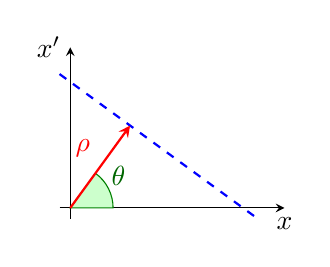
\begin{tikzpicture}[ 
    scale			= 0.68,
    %axis/.style		= {help lines, -{Stealth[length = 1.5ex]}},
    >=stealth
  ]
% axes
\draw[->] (-0.2,0) -- (4,0) node [below] {$x$};
\draw[->] (0,-0.2) -- (0,3) node [left] {$x'$};
% tilted line
\draw[-,blue, dashed, thick] (-0.2,2.5) -- (3.5,-0.2);
% angle
\filldraw[fill=green!20,draw=green!50!black] (0,0) -- (0.8,0) arc [start angle=0, end angle=54, radius=0.8] -- cycle;
% pointing arrow
\draw[->,red, thick] (0,0) -- node[above left]{$\rho$} (54:1.9);
% add some labels
\node[green!40!black] at (0.9,0.6) {$\theta$};
%
\end{tikzpicture}
\label{fig:tomoPhaseSpaceInitial}
%%%%%%%%%%%
}
% Start of second figure with circles
\,
%
\subfloat[]{ %[screen location]
%%%%%%%%%%%
\begin{tikzpicture}[ 
    scale			= 0.68,
    %axis/.style		= {help lines, -{Stealth[length = 1.5ex]}},
    >=stealth
  ]
% axes
\draw[->] (-0.2,0) -- (4,0) node [below] {$x$};
\draw[->] (0,-0.2) -- (0,3) node [left] {$x'$};
% tilted line
\draw[-,blue, dashed, thick] (2.5,-0.2) -- (2.5,3);
% pointing arrow
\draw[->,red, thick] (0,0) -- node[above]{$\rho'$} (0:2.5);
%
\end{tikzpicture}
\label{fig:tomoPhaseSpaceScreen}
}
\caption{
Correspondence between a phase-space profile integral line (dashed line) at the reconstruction location~\protect\subref{fig:tomoPhaseSpaceInitial} and at the measurement location~\protect\subref{fig:tomoPhaseSpaceScreen}.
The red arrows identify the distance of the integral line from the origin of the axes at the two locations.
}
\label{fig:tomoPhaseSpaces}
\end{figure}
%
Each point of a measured beam profile can be seen as a line integral over the
vertical-dashed line in
Fig.~\ref{fig:tomoPhaseSpaces}~\protect\subref{fig:tomoPhaseSpaceScreen}.
This is equal to the integral along the dashed line in
Fig.~\ref{fig:tomoPhaseSpaces}~\protect\subref{fig:tomoPhaseSpaceInitial}
representing the phase space at the reconstruction location. 
Assuming the linear transformation in Eq.~\ref{eq:simpleTranport}, the angle
$\theta$ and the relation between the distances $\rho$ and $\rho^{\prime}$
can be found to be:
%
\begin{align}
 \tan(\theta) &= \frac{B}{A} \qquad
 \rho' = \rho \sqrt{A^2 + B^2}.
\label{eq:tomographyRelations}
\end{align}
In practice each measured profile is a compressed projected distribution of
the beam phase space taken at different angles.
By carefully decompressing the profiles one can therefore use them for
reconstructing the actual beam phase-space distribution.
At CTF3 this is done by using the inverse Radon transformation provided by
MATLAB \cite{mat:radon}. 

Figure~\ref{fig:tomo} shows a typical measurement performed at CTF3 with an
heavily non-Gaussian beam.
%
%  using data file eh7365894873.dat
% angles moving from about 50 to about 170 deg.
\begin{figure}[htb]
   \centering
   \subfloat[]{ %[screen location]
   	\includegraphics*[width=0.49\columnwidth]{MOPAB115f4.eps}
   	\label{fig:tomoprofiles}
   } \\
   \subfloat[]{ %[screen location]
   	\includegraphics*[width=0.49\columnwidth]{MOPAB115f5.eps}
   	\label{fig:tomorec}
   }
   \caption{Measured horizontal beam profiles~\protect\subref{fig:tomoprofiles} used for the transverse
            phase-space tomographic reconstruction in~\protect\subref{fig:tomorec}.
            Dashed is the phase-space reconstruction using the simpler quadrupole
            scan technique.}
   \label{fig:tomo}
\end{figure}
%
Note the non-Gaussian profiles measured at the screen location 
in~\ref{fig:tomo}~\protect\subref{fig:tomoprofiles}, 
which are well exploited by the tomographic reconstruction but 
obviously ignored by the simple quadrupole scan reconstruction. 

